\chapter{基于对比学习的多项选择长文本阅读理解}
多项选择阅读理解旨在通过阅读并理解一篇给定的文章和问题,从多个备选答案中选出最合适的答案。
近期的研究致力于捕获文章、问题和选项三元组之间的联系。
然而,由于文本长度太长,模型很难重点关注备选答案之间的联系,最近的方法在面临复杂的多项选择问题时,往往会把干扰选项鉴别为正确答案。
鉴于人类往往通过比较备选答案之间的差异,来处理多项选择问题;受到这种现象的启发,本章提出CoLISA(对比学习和样本内注意力,Contrastive Learning and In-Sample Attention)模型,这是可以相对精准剔除干扰选项的新模型。
特别是CoLISA是通过在多个选项之间进行对比学习来获取蕴含其他选项信息的选项表示的。
此外,样本内注意力机制是应用于多个选项之间的,因此这些选项之间会彼此产生联系。
通过在两个多项选择数据集QuALITY和RACE上的实验结果表明,本章提出的CoLISA在正确与错误选项之间的联系花费了更多注意力,能够识别选项之间的差异。
同时,CoLISA也在QuALITY数据集上实现了SOTA(state-of-the-art)的性能。


\section{引言}
机器阅读理解(Machine Reading Comprehension,MRC)通过对给定文档进行推理,要求模型回答指定问题。
作为MRC任务中的变体之一,多项选择阅读理解\cite{richardson2013mctest}(Multi-choice Reading Comprehension,MC-RC)主要针对于在给定文章的情况下,从多个备选答案中选出最合适的答案,来回答问题。
MC-RC要求模型通过阅读并理解参考文章的前提下,来判别每个备选答案的正确性。

在MC-RC领域,现存的研究通常专注于针对给定问题,解决文章和备选答案之间的隔阂\cite{ran2019option,zhang2020dcmn+}。
这些模型对每个选项进行独立编码。
用这种方法,针对某个问题,每个选项并不能直观的与别的选项进行交互,这会限制模型的推理能力。
此外,在某些真实案例中,存在一些更棘手的情况。
对于一个特定的问题,某些备选答案在字面上,甚至在语义上都与正确答案很相近。换句话说,如果仅仅判别单个选项的正确性,它们很有可能都会被判定为正确的。
现存的方法也总是疏于处理这类例子。
本章认为,应该额外制定一种更精细的方法,来处理这些所谓的干扰项与正确答案之间的关系。
表~\ref{4-1}~具体描述了QuALITY\cite{pang2021quality}中一个关于难以辨别的干扰项的实例\footnote{QuALITY中也存在输入文章长度超过模型限制的情况,本章也会在后续讨论这个问题}。
参考例子中的整篇文章,可以认为正确答案$O_2$(加粗和加下划线)和干扰选项$O_1$(仅加下划线)可以认定都是接近于正确答案的。
为了根据给定问题选出最合适的答案,模型需要找到正确答案和干扰选项表示之间的差异。

\begin{table}[htbp]
    \centering
    \begin{tabular}{p{420pt}}
    \hline
    {\bfseries 文章:} \\
    (...) I'm sure that `justifiable yearnings for territorial self-realization' would be more appropriate to the situation (...) (Over 4,000 words) \\
    <译文:(...) 我确信“对领土自我实现的正当渴望”可能更适用于这种情况 (...) > \\
    \hline
    {\bfseries 问题:} \\
    According to Retief what would happen if the Corps did not get involved in the dispute between the Boyars and the Aga Kagans? \\
    <译文:如果Corps不介入Boyars和Aga Kagans的争端,根据Retief的说法会发生什么? > \\
    \hline
    {\bfseries 选项:} \\
    $O_1$: \textcolor[rgb]{0.4,0.7,0.9}{The Aga Kagans would enslave the Boyars} \\
    <译文:Aga Kagans会奴役Boyars> \\
    $O_2$: \textcolor[rgb]{1,0.4,0.3}{The Boyars and the Aga Kagans would go to war} \\
    <译文:Boyars和Aga Kagans会引发战争 > \\
    $O_3$: The Aga Kagans would leave Flamme to find a better planet \\
    <译文:Aga Kagans会离开Flamme,找到更好的星球> \\
    \textbf{$O_4$}: The Boyars would create a treaty with the Aga Kagans without the Corps' approval \\
    <译文:Boyars会与Aga Kagans签订条约,而不需要得到Corps的批准> \\
    \hline
    \end{tabular}
    \caption{\label{tab:4-1}
    QuALITY中的例子。
    }
\end{table}


人类总是需要通过仔细比较各个选项之间的差异,来排除看上去正确的错误选项,从而回答MC-RC问题\cite{daniel2017thinking}。
受到该流程的启发,本章提出了一个基于对比学习和样本内注意力(CoLISA)的架构,它包含两个主要的特性。
首先,由于应用了两次不同的dropout掩码,得到两个有着轻微差异的表示。也就是说,对于同一个输入,会有两组输出值,每一组都包含了一个正确答案和若干个错误选项。
CoLISA主要通过对比学习的方式,将两个正确选项的表示拉近,然后把正确答案与干扰选项之间的表示推远;因此,该模型可以学习到更有效的文本表示。
此外,自注意力机制\cite{vaswani2017attention}也应用在了特定样本中的多个选项之间,在选项之间共享彼此的信息。
所以,模型借助多个备选答案之间的自注意力交互的方式,学习到倾向于选择正确答案的能力。
本章也在两个MC-RC数据集QuALITY\cite{pang2021quality}和RACE\cite{lai2017race}上进行了实验。
实验结果表明,CoLISA的性能表现显著的超过了其他现存方法。
本章的贡献可以总结为如下:
\begin{itemize}
    \item[$\bullet$] 在多项选择长文本阅读理解任务中引入对比学习方法,用以辨别正确答案与干扰选项之间的差异。该方法通过分配更多的权重给干扰选项,使干扰选项获取到更多注意力。
    \item[$\bullet$] 针对一个特定的例子,通过将样本内注意力机制应用到多个选项之间,让它们彼此之间进行交互。
    \item[$\bullet$] 本章提出的方法CoLISA在QuALITY上实现了SOTA(state-of-the-art)的性能,并且在RACE上跟其他基线模型相比,也实现了可观的提升。
\end{itemize}


\section{基于对比学习的多项选择长文本阅读理解}
给定一篇参考文本,一个目标问题,还有一些备选答案,多项选择阅读理解(multi-choice reading comprehension, MC-RC)任务是指将其中一个选项预测为最终答案。
形式上来说,将一篇文章定义为$p=[s^p_1, s^p_2, ..., s^p_n]$,其中$s^p_i=[w^s_1, w^s_2, ..., w^s_l]$表示$p$中第$i$个句子,$w^s_j$表示$s^p_i$中的第$j$个词。
问题可以定义为$q=[w^q_1, w^q_2, ..., w^q_t]$,其中$w^q_i$表示$q$中的第$i$个词。
选项集合可以定义为$O=[o_1, o_2, ..., o_r]$,其中$o_i=[w^o_1, w^o_2, ..., w^o_k]$表示第$i$个选项,$w^o_k$表示$o_i$中第$k$个词。
MC-RC的目标是最大化所预测选项的概率:
\begin{equation}
    a = \argmax_i(\mathcal P(o_i|p,q)).
\end{equation}

当$p$的长度超过编码器的最大输入长度时,本章的做法是通过检索与问题和备选答案相关的句子,将长文本压缩成篇幅较短的文本。
较短文本表示为$c=[s^c_1, s^c_2, ..., s^c_m]$,其中$s^c_i=[w^s_1, w^s_2, ..., w^s_l]$表示$c$中的第$i$个句子,$w^s_j$表示$s^c_i$中的第$i$个句子。

\subsection{总体架构}
% 模型图
\begin{figure}[htbp]
    \centering
    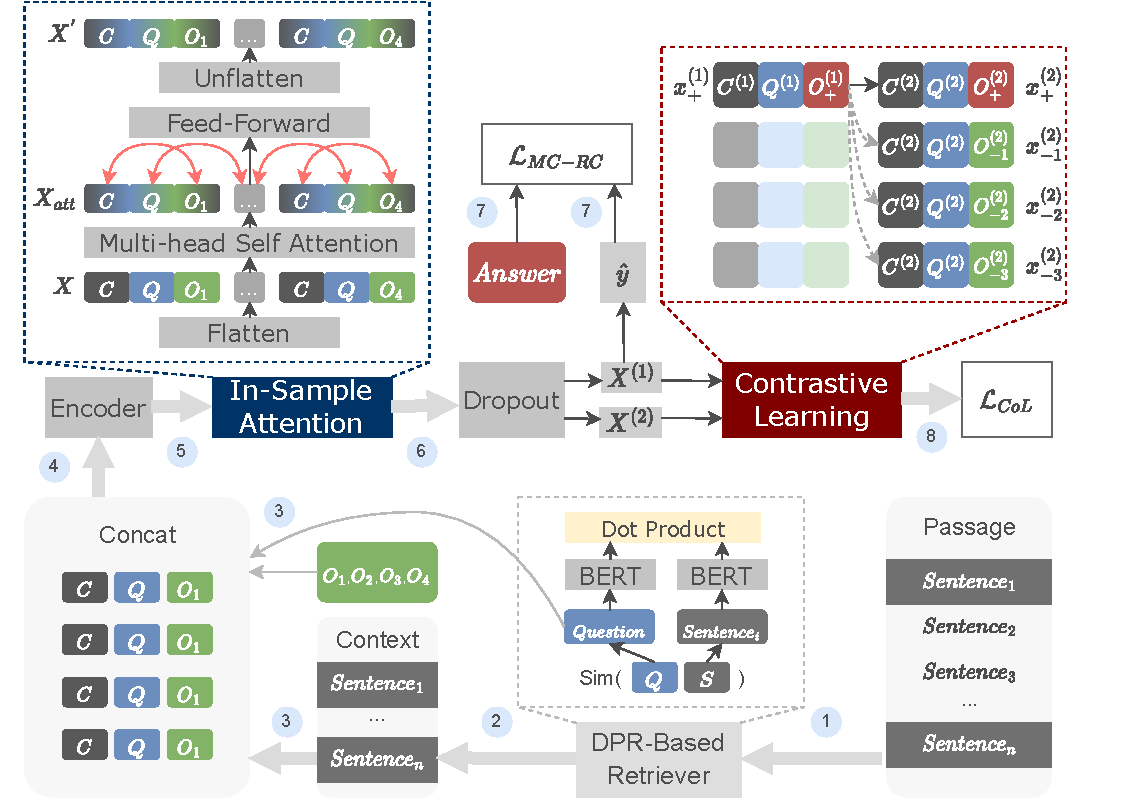
\includegraphics [width=1.0\textwidth] {figure/4-1.pdf}
    % \caption{The architecture of our model CoLISA. (1) A long passage is fed into the DPR-based retriever, (2) then comes out a shorter context, (3) together with a related question and multiple options in our dataset, they are (4) preprocessed and combined into four different sequences (in our dataset there are four options for each question), after going through the inherent (5) embedding and (6) encoder, these four sequences are represented as (7) vector representations, (8) followed by an ISA module listed on the right top of the figure, the sequences are flattened to a combined one, with multi-head self-attention across each token within the extended sequence, then the sequence roll back to the initial dimension, (9) the updated vectors are fed into a dropout twice to come out into two outputs, (10) one for calculating the cross-entropy loss (11) meanwhile both of them need feeding to a CoL module illustrated on the left top of the figure, to calculate a contrastive learning loss finally.}
    \caption{CoLISA的基本架构。} % Our proposed contrastive learning method and in-sample attention mechanism are highlighted boldly in dark red and dark blue rectangles, respectively.
    \label{fig:4-1}
\end{figure}

如图~\ref{fig:4-1}~所示,本章提出了一种新颖的MC-RC框架,它充分运用了对比学习和样本内注意力(contrastive learning and in-sample attention, CoLISA),主要由两部分组成:
首先是基于DPR(Dense Passage Retrieval,稠密检索)的检索器,在一篇很长的文章中,根据对给定问题和对应的过个备选答案之间的相关性,筛选出相关的句子,以此来根据原文的原始顺序来构建一段新的文本;
另外,CoLISA阅读器需要根据给定问题和上下文中,从若干选答案中预测出最终答案。
CoLISA阅读器由两部分组成。
第一部分是样本内注意力(In-Sample Attention, ISA)机制,换句话说,引入一个加入了多头自注意力机制并针对长序列的网络,来增强特定样本中多个选项之间的交互。
第二部分是对比学习(Contrastive Learning,CoL)以及一个干扰因子(Distractive Factor,DiF),来表示由上下文、问题和备选答案组合而成的序列。

\subsection{基于DPR的检索器}
为了从一篇长文本中筛选出相关的句子,本节首先使用了基于DRP(Dense Passage Retrieval,稠密检索)的句子检索器,该检索器常常用于隐式语义编码\cite{karpukhin2020dense}。
注意到两个来自DPR的编码器已经为抽取不同种类的句子提前做了预训练,本节使用了相应的DPR编码器来确保能检索到的句子的多样性。
上下文编码器$E_S$编码整个参考文章$p$中的所有句子$s$到$d$维的向量。
类似的,查询编码器$E_R$将问题$q$和选项集合$O$编码到$d$维的向量,作为两种不同的检索查询$r$。
$s$和$r$的[CLS]token的全局表示用于计算它们的负欧几里得距离($L^2$):
\begin{equation}
    -L^2_{dist}(r,s)=-||E_R(r)-E_S(s)||^2.
\end{equation}

对于选项查询,按照$s$和$r$之间的相关性的降序排序筛选出前$k$个句子。
同时,考虑到语义连贯性的问题,这$k$个句子的前一句和后一句也会筛选出来。
由于这种做法会导致同一个句子被多次选择,重复的句子将会只保留一遍。

对于问题查询,先得到前$n$个句子。\footnote{考虑到预训练语言模型能容纳所抽取的句子的总长度,$k$和$n$需要设定为合适的值,这里在所有实验中将$k$设为2,$n$设为1。}这里与选项查询仅仅存在一旦差异,因为针对本方法,来源于选项的证据相比于来源于问题的证据更合适,所以本节并没有采集前一句和后一句。
最终,潜在的重复句子已经消除,这样能确保所有抽取句子的唯一性。
在选出最合适的句子后,再根据原文顺序将这些句子进行排序,然后将他们拼接成一段参考上下文$c$。
算法~ref{alg:algorithm}~详细阐述了抽取的过程。

% \begin{algorithm}\small
%   \KwIn{Passage $p=[s_1, s_2, ..., s_n]$, Question $q$, Options $O=[o_1, o_2, ..., o_m]$}
%   \KwOut{Context}
%   \eIf{Input (x) belongs to p}{
%     $E_x$ = ContextEncoder($x$)\;
%     }{
%     $E_x$ = QuestionEncoder($x$)\;
%     % $E_o$ = QuestionEncoder($o$)\;
%     }
%   \For{$o_i$ in $O$}{
%     \For{$s_j$ in $p$}{
%       sim($o_i$, $s_j$) = -L^2_{dist}($E_{o_i}$, $E_{s_j}$)
%       }
%     Select: Top-k relevant sentences $s_{i_1}, s_{i_2}, ..., s_{i_k}$\;
% 	Select: Their previous and next sentences $s_{i_1}^{prev}, s_{i_1}^{next}, ..., s_{i_k}^{prev}, s_{i_k}^{next}$\;
% 	Context $\gets$ Selected sentences\;
% 	}
%   \For{$s_j$ in $p$}{
%     sim($q$, $s_j$) = -L^2_{dist}($E_q$, $E_{s_j}$)
% 	}
%   Select: Top-n relevant sentences $s_{j_1}, s_{j_2}, ..., s_{j_n}$\;
%   Context $\gets$ Selected sentences\;
%   Context.unique().sort().to\_str()\;
%   \caption{\label{alg:algorithm}The Extracting Algorithm}
% \end{algorithm}


\begin{algorithm}\small
  % \KwIn{Passage $p=[s_1, s_2, ..., s_n]$, Question $q$, Options $O=[o_1, o_2, ..., o_m]$}
  % \KwOut{Context}
  % \eIf{Input (x) belongs to p}{
  %   $E_x$ = ContextEncoder($x$)\;
  %   }{
  %   $E_x$ = QuestionEncoder($x$)\;
  %   % $E_o$ = QuestionEncoder($o$)\;
  %   }
  % \For{$o_i$ in $O$}{
  %   \For{$s_j$ in $p$}{
  %     sim($o_i$, $s_j$) = -L^2_{dist}($E_{o_i}$, $E_{s_j}$)
  %     }
  %   Select: Top-k relevant sentences $s_{i_1}, s_{i_2}, ..., s_{i_k}$\;
	% Select: Their previous and next sentences $s_{i_1}^{prev}, s_{i_1}^{next}, ..., s_{i_k}^{prev}, s_{i_k}^{next}$\;
	% Context $\gets$ Selected sentences\;
	% }
  % \For{$s_j$ in $p$}{
  %   sim($q$, $s_j$) = -L^2_{dist}($E_q$, $E_{s_j}$)
	% }
  % Select: Top-n relevant sentences $s_{j_1}, s_{j_2}, ..., s_{j_n}$\;
  % Context $\gets$ Selected sentences\;
  % Context.unique().sort().to\_str()\;
  \caption{\label{alg:algorithm}The Extracting Algorithm}
\end{algorithm}


\subsection{样本内的自注意力机制}
当编码$q$和$o_i$时,对于同一个问题,不同选项的编码相互之间都是独立的,这样就就导致了这些备选答案之间的注意力缺失。
为了解决这个问题,本章借鉴了人类回答多项选择问题的方式。
一般来说,一个人会通过同时比较多个选项来排除干扰项,最终决定该选择哪个选项。
受到这种方式的启发,本章提出了一种样本内的注意力(In-Sample Attention,样本内注意力)机制,来增强不同选项表示之间的交互作用。

通常,每个别选答案$o_i$先和它对应的上下文$c$以及问题$q$进行拼接,构成一个三元组$x_i=[c;q;o_i]$。
本章通过将每个$x_i$依次喂入预训练编码器中,从而得到一系列完整的序列表示。
为了建模多个选项$o_i$之间的联系,本章提出的ISA模块首先收集到所有与相同问题$q$对应的$x_i$,对它们进行拼接,构建一个单独的序列$X=[x_1;x_2;...;x_n]$。
然后,计算$X$的自注意力表示,来学习多个选项之间的远程依赖。
具体来说,利用平凡的自注意力机制的架构,同时将序列$X$分解为三个矩阵$Q$,$K$,$V$。
输出的自注意力矩阵可以计算为:
\begin{equation}
    SA(Q,K,V)=softmax(\frac {QK^T}{\sqrt{d_k}})V,
\end{equation}
其中$d_k$是一个缩放因子,它表示$K$的维度,以防引起梯度消失现象\cite{vaswani2017attention}。
更进一步,多头注意力机制被引入到ISA中,从不同的向量维度来更加综合性的表示$X$。
多头自注意力的流程可以定义为:
\begin{align}
    & head_i = SA(QW^Q_i,KW^K_i,VW^V_i), \\
    & H = Concat(head_1,...,head_h), \\
    & MSA(Q,K,V) = HW^O,
\end{align}
其中$h$表示各个平行注意力头的数量,$W^Q_i,W^K_i,W^V_i,W^O$是注意力参数矩阵。
这里还将多头自注意力的向量表示记为$X_{att}$。
如图~ref{4-1}~中的ISA机制所描述的,作用在拼接后的序列$X$的注意力机制通过计算选项之间的表示$X_{att}$,实现彼此之间的交互。

此外,为了避免多头自注意力输出的塌陷\cite{vaswani2017attention,sukhbaatar2019augmenting},多头自注意力机制后面还增加了一个全连接网络:
\begin{equation}
    X_{ffn}=FFN(X_{att}).
\end{equation}
这里使用了GeLU\cite{hendrycks2016gaussian}函数作为激活函数。
最终,$X_{fnn}$需要根据多个输入三元组$x_i$的维度拆解为多个表示。
输出三元组的结合记为$X^{'}$。

\subsection{用于备选答案交互的对比学习方法}
为了鼓励CoLISA能够显式区分正确答案和干扰选项的表示之间的差异,本节引入了对比学习(Contrastive Learning,CoL)模块。
受到通用的对比学习框架\cite{gao2021simcse}的启示,CoL模块旨在促进两个正向三元组的表示变得更接近,而将同一样本内的所有表示均匀的分布在特定的向量空间上。
紧接着上一节的ISA模块之后,具有交互注意力的输入向量$X^{'}$被传递到dropout层,并执行同样的操作两次,来针对每个输入产生两个有轻微差异的的编码表示,记为$X^{(1)}$和$X^{(2)}$。

之后,先要计算MC-RC任务中在目标标签$y$和输出$X^{(1)}$之间的交叉熵损失。
具体来说,通过一层全连接神经网络可以将$X^{(1)}$转换为预测输出$\hat y$,它的维度与标签$y$相同。
损失函数定义如下:
\begin{equation}
    \begin{split}
    \mathcal L_{MC-RC}=& -\frac{1}{N}\Sigma^N_{i=1}(y^{(i)}\log\hat y^{(i)}+(1-y^{(i)})\log(1-\hat y^{(i)})).
    \end{split}
\end{equation}
注意到来自于同一样本的$X^{(1)}$和$X^{(2)}$都是由相同数量的三元组$x_i$组成的:一个包含正确答案的三元组和剩余的包含错误答案的三元组。
因此,对于每个输入样本中的两个输出结果,对比损失定义为负对数似然函数的平均值。
更具体来讲,对于其中一个输出$X_{(1)}$,本节将含有正确答案的三元组作为锚点,同时移除了包含错误选项的三元组。针对另一个输出$X_{(2)}$,所有的三元组都被保留了下来:其中含有正确选项的三元组视为正例,其他三元组被视频负例。
每个损失项可以区分正例和负例的差异。
CoL的损失函数定义如下:
\begin{equation}
    \mathcal L_{CoL}=-\frac{1}{N}\Sigma^N_{j=1}\log \frac{e^{sim(x^{(1)}_+,x^{(2)}_+)/ \tau}}{\Sigma^S_{i=1} e^{sim(x^{(1)}_+,x^{(2)}_i)/ \tau}},
\end{equation}
其中$x^{(1)}_+$是$X^{(1)}$中包含正确答案的三元组的编码表示,而$x^{(2)}_i$是$X^{(2)}$中所有三元组的表示,$X^{(2)}$中的$x^{(2)}_+$是正例样本,$\tau$是可配置的超参数,温度系数。
$sim(\cdot)$是一种相似度指标(本章中所有的实验都是使用余弦相似度函数),$S$代表了每个样本中三元组的数目,$N$代表了batch的大小。
聚合后的对比损失$\mathcal L_{CoL}$主要通过在每个batch中的所有样本取平均获得。

\noindent \textbf{Distractive Factor.}
基于样本中不同的干扰项会对模型造成不同程度的干扰,本节还将一个对比因子(Distractive Factor, DiF)引入到了CoLISA模型,具体来说,将DiF结合到对比学习的过程当中。
QuALITY的数据标注人员针对每个问题的所有错误选项中,把误导他们最严重的的那个标记为强干扰项。
因此,本节中通过构建一组置信因子,根据每个选项对应的标注分数,来代表它们对$\mathcal L_{CoL}$的贡献度。
本节中枚举了对每个选项的标注票数来构建DiF $\Theta=[\theta_1, \theta_2, ..., \theta_n]$,其中$n$是备选答案的数量。
然后再用一个softmax函数来帮助缩放$\Theta$,从而更明显的区分每个$\theta_i$。
每个$\theta_i$被修正为如下的形式:
\begin{equation}
    \theta_i=\frac{e^{\theta_i}}{\Sigma^n_i e^{\theta_i}}.
\end{equation}
幂运算可以清晰的却分$n$个系数$\theta_i$。
当计算对比损失的时候,$\theta_i$乘上了它对应选项的相似度的值,来衡量正确答案和干扰答案的差距。
$\theta_i$的值越大,对对应选项贡献的损失就越多。
经过上述分析,对比损失函数可以改进为如下:
\begin{equation}
    \mathcal L_{CoL}=-\frac{1}{N}\Sigma^N_{j=1}log \frac{\theta_+e^{sim(x^{(1)}_+,x^{(2)}_+)/ \tau}}{\Sigma^S_{i=1} \theta_ie^{sim(x^{(1)}_+,x^{(2)}_i)/ \tau}},
\end{equation}
其中$\theta_+$和$\theta_i$分别对应样本中的正例以及第$i$个选项。
最终的损失函数可以表示为:
\begin{equation}
    \mathcal L=\alpha \cdot \mathcal L_{MC-RC}+(1-\alpha) \cdot \mathcal L_{CoL},
\end{equation}
其中$\alpha \in[0,1]$是一个平衡系数。


\section{实验及结果分析}
本节首先描述了实验设置,然后提供实验及其对应结果。
然后又进一步描述了与其他现存模型的对比,并做了一些消融实验。

\subsection{实验设置}
本节使用了基准数据QuALITY和RACE来评估CoLISA模型的效果。
最主要的实验是在QuALITY上进行的\footnote{基于DPR的检索器对于QuALITY中的长文本输入是可行的。此外,最强干扰项只在QuALITY中有标注,因此,大部分实验都在QuALITY上完成。},同时也报告了RACE上的其他实验结果。

\begin{itemize}
    \item QuALITY~\cite{pang2021quality}. 
        这是一个多项选择阅读理解(MC-RC)数据集,其每篇文章的平均长度大约有5000个token。
        该数据集中最值得一提的特征是,一些干扰选项会对模型的认知能力造成负面影响。
        如果不依靠摘要或者文本片段,略读和简单的搜索不再足以让模型持续表现出优异的性能。
        数据集中的文中主要采集于科幻小说和杂志,并且标注人员都对其进行了阅读和评估。
    \item RACE~\cite{lai2017race}.
        鉴于QuALITY只由6,737条源数据构成,这难以全面的评估实验结果,因此实验中还利用到了另一个大规模MC-RC数据集,来验证模型的性能。
        RACE数据集从中国的中考和高考英语阅读理解试题进行收集。
        大多数问题也需要推理。
        此外,文本涉及的领域是多样的,从新闻、故事到广告,这让数据集也更加具有挑战性。
\end{itemize}

针对QuALITY\cite{pang2021quality}和RACE\cite{lai2017race}两大数据集,本章主要使用准确率(acuracy, acc)作为评估标准,来衡量问题回答正确的比例。
由于两个数据集中都存在不同难度的文本,本章中的主要实验也使用了QuALITY中全部/困难子集的$acc$,以及RACE\footnote{QuALITY中的源数据根据问题难度分为全部和困难子集,而在RACE中,中考和高考子集代表了两个水平的入学考试试题。}中中考/高考子集的$acc$。
对于基于DPR的检索器,本节使用了和QuALITY中的基线模型中的相同的方法,来减缓检索稀疏性的影响,从而做一个公平比较。
详细来说,本节使用了一个问题编码器来编码查询输入,以及一个上下文编码器来编码文章。

对于CoLISA的阅读器,本节主要使用了DeBERTaV3-large模型作为预训练语言模型。
对于所有实验,在QuALITY和RACE上训练时的学习率为1e-5,热身率为0.1。
Dropout比例保持为了默认的0.1,激活函数使用的是GeLU\cite{hendrycks2016gaussian}。
所有实现都使用了16的batch尺寸,以及512个token的最大长度。
模型微调在QuALITY上进行了20轮,RACE上进行了3轮。

对于对比学习部分,由于实验开销的原因,本节在DeBERTaV3-base和RoBERTa-base模型上调整温度系数$\tau$。
经调参后,基础模型上最优的$\tau$值0.1直接应用于大模型中。
同时,交叉熵损失和对比损失分别分配一半到最终的综合损失中。
此外,先前提到的干扰因子仅仅应用于QuALITY的实验中,因为RACE数据集没有对所有选项进行干扰程度标注。

所有实验都在一张Tesla V100-32GB的GPU上进行训练,Apex中的fp16精度模式也用于加速训练过程。

尽管在QuALITY上由很多方法可以进行尝试,本章仅仅选取了两个典型的基线模型。

\begin{itemize}
    \item Longformer~\cite{beltagy2020longformer}. 
        该预训练语言模型结合了滑动窗口局部注意力和全局注意力机制,来编码较长的文本序列。
        Longformer支持最多达到4,096长度的输入序列。
        实验对比过程中采取了Longformer作为其中一个基线模型,因为它包含了需要回答QuALITY样本中大部分的文本。
    \item DPR \& DeBERTaV3~\cite{karpukhin2020dense,he2021debertav3}。
        该管道架构由一个检索器和一个阅读器组成。
        基于DPR的检索器用于在一篇文章中针对指定问题抽取最相关的上下文。
        被选取的上下文作为输入的一部分,将被喂给后续的模块。
        最后,一个用于MC-RC标准的DeBERTa-V3模型将会抉择出正确的答案选项。
\end{itemize}

\subsection{实验结果和分析}

\begin{table}\scriptsize
    \centering
    \begin{tabular}{ll|ll|ll|ll}
    \hline
    {\bfseries Model} & {\bfseries Acc} & {\bfseries Model} & {\bfseries Acc} & {\bfseries Model} & {\bfseries Acc} & {\bfseries Model} & {\bfseries Acc} \\
    \hline
    Baseline & 56.7 & Baseline & 56.7 & Baseline & 56.7 & Baseline & 39.6 \\
    \hline
    CoL & {\bfseries 60.1} & CoL & 60.1 & CoL & 60.1 & CoL & {\bfseries 40.8} \\
    \hline
    $\ $ question query & 58.9 & $\ $ w/ DiF & {\bfseries 60.9} & $\ $ w/ self-attention & 60.4 & $\ $ in-batch negatives & 37.1 \\
    $\ $ in-batch negatives & 59.4 & $\ $ KL Loss & 57.0 & $\ \ $ context masked & 60.4 & \\
    & & & & $\ $ w/ transformer & {\bfseries 61.0} & & \\
    & & & & $\ $ w/ transformer*2 & 60.8 & & \\
    & & & & $\ $ w/ modified transformer & 58.9 & & \\
    \hline
    \end{tabular}
    \caption{\label{tab:4-3}
    Ablation study on contrastive learning module, distractive factor, and in-sample attention mechanism on the development set of QuALITY.
    }
\end{table}


本节将CoLISA模型与两个QuALITY上强力的基线模型进行比较,以及RACE上三个预训练语言模型进行比较。
整体结果如表~\ref{tab:4-3}~上所显示,CoLISA超越了其他所有的模型。
Longformer性能的匮乏说明了Longforemr并不擅长在一段冗长的源文本上定位关键信息。
具体原因极有可能是长文本预训练语言模型需要更多的训练数据,而QuALITY给出的训练数据十分有限。
此外,QuALITY中文本的长度仍旧超过了Longformer的最大编码长度限制,这可能会引起关键信息的损失。
相比之下,DPR \& DeBERTaV3架构由于自身的抽取策略,其性能表现更突出。
同之前提到的两个基线模型相比较,CoLISA学习到了更有效的上下文表示方法,并通过引入的对比学习(CoL)策略,更加准确的识别多个备选答案之间的差异。
同时,在DeVERTaV3的编码器之后加入样本内注意力(ISA)机制,会持续增强模型的性能表现。
这种尝试意味着,用一种ISA风格的方式在多个选项之间进行内部交互,会进一步捕捉到所有备选答案之间的差异关系。


\subsection{实验分析}

\begin{table}\scriptsize
    \centering
    \begin{tabular}{ll|ll|ll|ll}
    \hline
    {\bfseries Model} & {\bfseries Acc} & {\bfseries Model} & {\bfseries Acc} & {\bfseries Model} & {\bfseries Acc} & {\bfseries Model} & {\bfseries Acc} \\
    \hline
    Baseline & 56.7 & Baseline & 56.7 & Baseline & 56.7 & Baseline & 39.6 \\
    \hline
    CoL & {\bfseries 60.1} & CoL & 60.1 & CoL & 60.1 & CoL & {\bfseries 40.8} \\
    \hline
    $\ $ question query & 58.9 & $\ $ w/ DiF & {\bfseries 60.9} & $\ $ w/ self-attention & 60.4 & $\ $ in-batch negatives & 37.1 \\
    $\ $ in-batch negatives & 59.4 & $\ $ KL Loss & 57.0 & $\ \ $ context masked & 60.4 & \\
    & & & & $\ $ w/ transformer & {\bfseries 61.0} & & \\
    & & & & $\ $ w/ transformer*2 & 60.8 & & \\
    & & & & $\ $ w/ modified transformer & 58.9 & & \\
    \hline
    \end{tabular}
    \caption{\label{tab:4-4}
    Ablation study on contrastive learning module, distractive factor, and in-sample attention mechanism on the development set of QuALITY.
    }
\end{table}


\noindent \textbf{对比学习。}
为了有效评估CoL模块是如何影响整个模型表现的,本节中完成了一个消融实验,具体如表~ref{tab:4-4}~中的第一列所示。
首先,在抛弃ISA模块的情况下,可以评估只使用对比学习的方法会导致如何影响模型整体的性能。
实验结果可以证实,相比于基线模型,单独运用CoL组件的方法会显著提升模型性能,这里的基线模型是指表中前三列DPR \& DeBERTaV3-large的架构。

对于基于DPR的检索器,CoL让问题和多个备选答案都作为查询词,来从参考文章中抽取上下文。
作为对比,如果仅仅使用问题作为查询词,会导致性能有大幅度的下降。
这里给出的解释是,CoL方法主要针对于将正确答案和干扰选项之间进行区分,这样就可以更好的抽取于问题/备选答案相关的证据文本。

通过使用标准的dropout两次,可以得到两个不同的语义文本的表示。
在对比学习的过程中,每一个表示分别包含了一个正例。
在收集负例的时候,先前的工作会将同一个batch中剩余的样本视为负例,通常称之为batch内的负例\cite{gao2021simcse}。
本节也测试了一下batch内负例的方法。
遵循这种方法,实验结果揭示,将构建负例的方法从样本内部改为batch内部,会导致性能下跌\footnote{事实上,基础模型上的性能远远低于表格中列出的,当把相同的实验从大模型迁移到基础模型时,会表现出更差的性能。结果列在了表~ref{tab:4-4}~的最后一列中。性能从40.8疯狂跌到37.1。这里的基线模型是RoBERTa-base。对于大模型,由于机器设备的限制,实验中不得不使用一个较小的batch尺寸。因此,在大模型上无论是batch内的方法还是样本内的方法,都不能展示出巨大的差异。}。
在同一个batch内,多个样本之间没有必然的联系,这就违背了将正确答案按和干扰选项推远的目标。

\noindent \textbf{干扰因子。}
正如之前所提到的,CoLISA中设计了一个专门针对QuALITY的干扰因子(Distractive Factor, DiF);来强调困惑选项的作用。
表~ref{tab:4-4}~中的第二列展示了有关DiF的实现结果,其中本节中将DiF $\Theta$与对应选项的相似度进行相乘操作,来体现对干扰项的权重。
从实验结果中可以观察到,DiF这项操作显著增强了CoL模块的性能。
一个直观的解释是,DiF迫使干扰选项为对比损失贡献更多的数值,使模型更倾向于去学习如何识别干扰选项。

出于一种假设,每个备选答案成为最终答案的可能性遵循一种特定的概率各分布,本节在进行实验时,直觉上将KL散度损失~\ref{hershey2007approximating}~替换掉原来的交叉熵损失。
通过骤降的结果表明,KL散度展现出的功能与DiF比较相似。
同时,交叉熵损失对于辨别每个拼接上上下文、问题和备选答案的三元组的正确性是不可或缺的。

\noindent \textbf{样本内注意力。}
如表~\ref{tab:4-4}~中的第三列所示,本节中还利用了ISA机制的变体来验证它们的有效性。
可以如预期中观察到,当ISA机制是自注意力机制时,实验性能会由于多个三元组之间存在交互而提升。
然后,实验进一步尝试去遮蔽上下文token,这就意味着只有问题与选项彼此之间可以进行注意力交互,并没有上下文信息的参与。
结果性能是维持不变,这表明问题和备选答案之间的注意力交互是关键的步骤。

消融实验也进一步展示了transformer架构优于单独的一层自注意力层。
这是因为,transformer内部的前馈网络保留了大量的参数,来确保注意力输出的传播。
另有一个有趣的现象,如果再配上额外的一层transformer层,会导致模型性能轻微的下降。
本节认为,从RACE和QuALITY上先后微调的checkpoint被继续沿用,扩充了随机初始化的参数,这会加重训练负担。

此外,本节还通过移植编码器内部的注意力机制,修改了基础编码器的内部结构。
整个预训练编码器由$n$层\footnote{对于基础模型,$n$是12;对于大模型,$n$是24。}组合而成,其中每一层共享完全相同的结构:一个多头自注意力子层和一个前馈神经网络子层。
接下来,本节也针对多项选择的交互,尝试在两个子层之间增加了一个额外的注意力层。
注意到,更低的层主要表达浅层的语义,而更高的层主要针对深层语义,实际操作中只在在顶端的4层补充了注意力机制。
这种修改过后的transformer架构直觉上建模了低层次中的序列内交互,以及高层次中的多序列交互。
实验结果表明,修改编码器架构并不是最好的方法,因为这么做并没有完全利用预训练的成果。


\section{本章小结}
本章针对多项选择长文本阅读理解,通过对比学习方法和样本内注意力机制的方法,专注于处理备选答案中的干扰选项。
本章中提出的方法CoLISA,实现了多个选项之间的交互,从而解决迫切需要在正确答案和干扰选项之间进行严谨对比的困难样例。
CoLISA相关的实验在两个不同的基准数据集上都实现了持续的性能提升。
对于未来工作,可能会去探索对比学习方法更多相关的变体。


